% !TeX program = xelatex
% =====================================================================
%  “华为杯”第二十三届中国研究生数学建模竞赛 · 论文主文件
%  章节结构：1 问题重述｜2 问题分析｜3 模型假设与关键符号说明｜4 数据提取与预处理
%            5 问题一｜6 问题二｜7 问题三｜8 问题四｜9 模型评价与推广｜参考文献｜附录A
%  编译链（必须按顺序）：xelatex main.tex  →  bibtex main  →  xelatex main.tex ×2
%    第 1 遍 xelatex：生成 .aux（引用键清单）
%    bibtex main    ：读 gmcm.bst 生成 main.bbl（按引用顺序编号）
%    后 2 遍 xelatex：写入参考文献与交叉引用
%  （若只写纯文本、不引参考文献，可只跑 xelatex ×2）
% =====================================================================
\documentclass{huawei-cup}

% ===== 仅在此处填写参赛信息（只允许出现在封面）=====
\renewcommand{\paperschool}{某某大学}
\renewcommand{\teamnumber}{123456789}
\renewcommand{\memberone}{张三}
\renewcommand{\membertwo}{李四}
\renewcommand{\memberthree}{王五}
\renewcommand{\papertitle}{基于某某模型的某某问题研究}
\keywords{数学建模；关键词二；关键词三；关键词四}

\begin{document}

% 封面不显示页码；参赛信息只允许出现在封面。
\maketitlepage

% 摘要页从第 1 页开始计页码，摘要通常不超过两页。
\begin{abstract}
本文针对某某问题，首先说明研究对象、数据来源与任务目标；随后概括数据预处理、模型构建、参数求解和模型检验的完整思路。

针对问题一，建立某某模型，得到主要结果与误差指标。针对问题二，在前述模型基础上引入某某约束，并通过敏感性分析或稳健性检验说明结论的可靠性。针对问题三，构建某某优化模型，给出可复现的求解方案及关键数值结果。针对问题四，给出某某预测或分解结果，并说明其适用条件与不确定性。

最后概括模型的创新点、适用范围与局限性。摘要应写出具体方法、模型、结果、结论和创新点，避免只复述题目或罗列章节。
\end{abstract}

% 摘要页的下一页开始正文。
\section{问题重述}
用自己的语言准确重述问题背景、已知条件和各子问题任务，避免大段照抄题面。正文不得出现学校、队员姓名、指导教师等身份信息。

\section{问题分析}
说明各子问题之间的逻辑关系、可利用的数据、拟采用的方法以及预期输出。

\subsection{问题一分析}
给出从数据到模型再到评价指标的分析链条。

\subsection{问题二分析}
说明该问题相对问题一新增的约束、信息或决策变量。

\subsection{问题三分析}
说明本问的决策变量、预算或资源约束，以及与前两问输出的衔接关系。

\subsection{问题四分析}
说明本问的时间轴、评价口径与不确定性来源，并声明哪些结论只作情景外推。

\section{模型假设与关键符号说明}
\subsection{模型假设}
\begin{enumerate}[label=\arabic*.,leftmargin=2em,itemsep=0pt]
  \item 假设一，并说明作出该假设的现实依据；
  \item 假设二，并说明其对模型适用范围的影响；
  \item 假设三。\label{assumption:three}
\end{enumerate}
只列对结论有实质影响的假设；与后文无关的通用假设不必罗列。

\subsection{关键符号说明}
\begin{table}[H]
  \centering
  \caption{主要符号说明}
  \label{tab:symbols}
  \begin{tabular}{ccc}
    \toprule
    符号 & 含义 & 单位 \\
    \midrule
    $x_i$ & 第 $i$ 个决策变量 & -- \\
    $y_i$ & 第 $i$ 个观测值 & -- \\
    $n$   & 样本数量 & 个 \\
    \bottomrule
  \end{tabular}
\end{table}
表中只保留后文反复使用的关键符号，其余符号在首次出现处随文说明。

\section{数据提取与预处理}
交代数据的提取口径与清洗流程。本节的输出是后面四问共用的输入，避免在各问中重复描述。

\subsection{数据来源与读取方式}
列出所用附件编号（如 A1--A3、B1--B5、C8 等）与实际读取方式；大文件须说明流式或分块读取，并给出处理后的记录数。

\subsection{清洗口径与指标方向统一}
说明缺失值、异常值、重复记录的处理规则与量纲统一方式。质量类指标必须统一转换为“越高越好”，并说明转换函数与依据\cite{ref-journal}。

\subsection{数据划分与泄漏控制}
说明训练/验证/测试或时间回测的划分方式、样本单位与分组键，并明确哪些信息在划分之后才可使用，避免信息泄漏\cite{ref-book}。

\section{问题一的模型建立与求解}
\subsection{模型建立}
给出目标函数与约束的完整形式。例如
\begin{equation}
  \min_{\boldsymbol{x}}\; f(\boldsymbol{x})
  = \sum_{i=1}^{n}\bigl(y_i-\hat y_i(\boldsymbol{x})\bigr)^2,
  \label{eq:objective}
\end{equation}
其中，符号含义见表~\ref{tab:symbols}。公式、图、表均应先在正文中引用，再出现相应对象。

\subsection{求解算法}
算法~\ref{alg:demo}给出求解流程；数据字段口径依据公开说明文档\cite{ref-web}。

% ---------- 【示例 1】算法伪代码（可直接复制，改内容即可）----------
\begin{algorithm}[H]
  \caption{分层求解流程（示例）}
  \label{alg:demo}
  \begin{algorithmic}[1]
    \REQUIRE 观测数据 $\{(x_i,y_i)\}_{i=1}^{n}$，预算上限 $B$
    \ENSURE 最优配置 $\boldsymbol{x}^{*}$ 与目标值 $f^{*}$
    \STATE 初始化参数 $\boldsymbol{x}^{(0)}$，令迭代计数 $k \leftarrow 0$
    \WHILE{未达到收敛条件}
      \STATE 计算当前点梯度 $\nabla f(\boldsymbol{x}^{(k)})$
      \IF{当前点不可行}
        \STATE 投影回可行域
      \ELSE
        \STATE 沿可行方向更新 $\boldsymbol{x}^{(k+1)}$
      \ENDIF
      \STATE $k \leftarrow k+1$
    \ENDWHILE
    \RETURN $\boldsymbol{x}^{(k)}$
  \end{algorithmic}
\end{algorithm}

\subsection{求解结果与检验}
报告关键参数、主要结果和评价指标，并说明检验方案。图~\ref{fig:subfig-demo}展示子图排版，表~\ref{tab:longtable-demo}展示跨页长表排版。

% ---------- 【示例 2】子图（subcaption：自动生成 (a)(b) 标号）----------
\begin{figure}[H]
  \centering
  \begin{subfigure}[b]{0.47\textwidth}
    \centering
    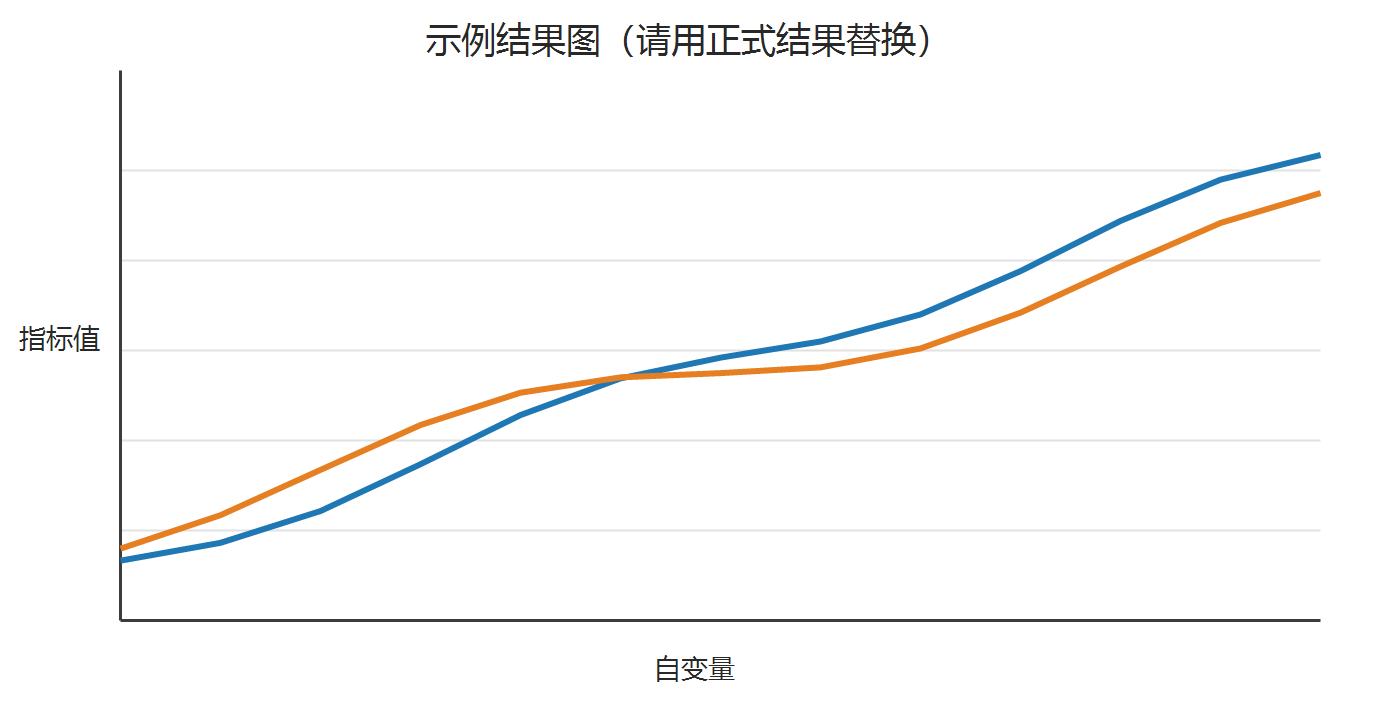
\includegraphics[width=\linewidth]{figures/example-result.png}
    \caption{结果一}
    \label{fig:sub-a}
  \end{subfigure}\hfill
  \begin{subfigure}[b]{0.47\textwidth}
    \centering
    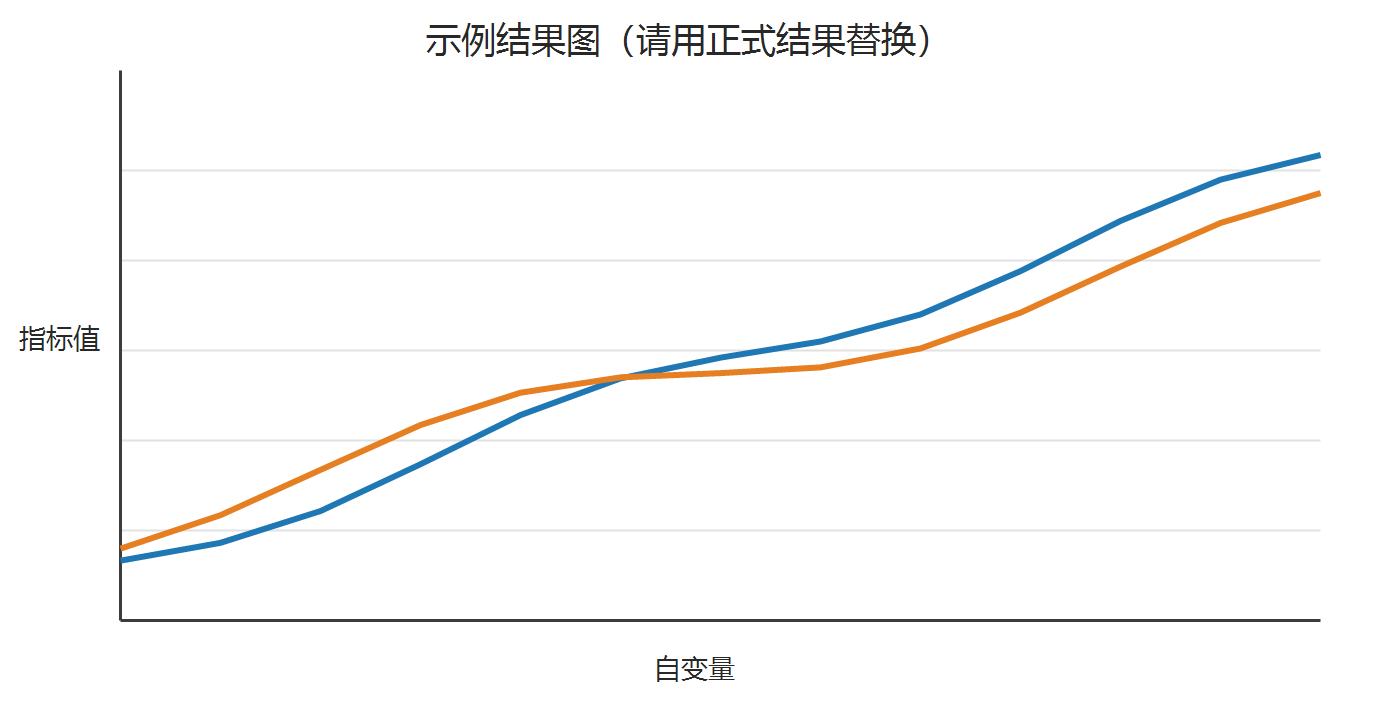
\includegraphics[width=\linewidth]{figures/example-result.png}
    \caption{结果二}
    \label{fig:sub-b}
  \end{subfigure}
  \caption{子图排版示例；正文先引用图~\ref{fig:sub-a}、图~\ref{fig:sub-b}，再解释差异}
  \label{fig:subfig-demo}
\end{figure}

% ---------- 【示例 3】跨页长表（longtable：表头自动重复）----------
\begin{longtable}{cccc}
  \caption{长表格排版示例（跨页时表头自动重复）}
  \label{tab:longtable-demo}\\
  \toprule
  序号 & 参数 & 取值 & 单位 \\
  \midrule
  \endfirsthead
  \multicolumn{4}{l}{\small 续表~\thetable}\\
  \toprule
  序号 & 参数 & 取值 & 单位 \\
  \midrule
  \endhead
  \bottomrule
  \endlastfoot
  1 & 学习率 & 0.001 & -- \\
  2 & 迭代上限 & 500 & 次 \\
  3 & 正则系数 & 0.05 & -- \\
  4 & 训练集比例 & 0.70 & -- \\
  5 & 验证集比例 & 0.15 & -- \\
  6 & 测试集比例 & 0.15 & -- \\
\end{longtable}

\section{问题二的模型建立与求解}
按照“模型目标—变量与参数—约束条件—求解算法—结果分析—模型检验”的顺序撰写。

\section{问题三的模型建立与求解}
写明决策变量、约束与预算情景；先给出可行解，再报告优化结果，并说明单位制与约束校验方式。

\section{问题四的模型建立与求解}
写明时间轴、口径与分解方式；预测或外推结果须给出不确定区间与适用条件。

\section{模型评价与推广}
\subsection{模型优点}
结合题目与结果说明，不写空泛表述。

\subsection{模型局限性}
说明数据、假设、算法复杂度或外推范围方面的限制。

\subsection{模型推广}
说明模型能够迁移到哪些场景，以及需要增加哪些数据或约束。

% ---------- 参考文献：BibTeX（gmcm = GB/T 7714 数字制，按引用顺序编号）----------
\bibliographystyle{gmcm}
\bibliography{reference}

\appendix
\ctexset{section={name={附录,},number=\Alph{section},aftername=\quad}}
\section{程序代码与补充材料}
按赛题与竞赛系统要求上传计算结果和源程序；仅在论文附录中保留必要的关键算法、补充推导或结果说明。引用他人程序时必须注明来源。

% ---------- 【示例 4】源码清单（listings：中文注释可正常显示）----------
\begin{lstlisting}[language=Python,caption={关键求解代码（节选，示例）},label={lst:code-demo}]
# 这是示例程序，请替换为真实运行过的代码；本行是中文注释，用于检查中文渲染
import numpy as np
from scipy.optimize import minimize

def objective(x, y):
    """目标函数：残差平方和"""
    return float(np.sum((y - model(x)) ** 2))

def solve(y, x0):
    res = minimize(objective, x0, args=(y,), method="L-BFGS-B")
    return res.x, res.fun

if __name__ == "__main__":
    x_opt, f_opt = solve(np.array([1.0, 2.0, 3.0]), np.zeros(3))
    print("最优解:", x_opt, "目标值:", f_opt)
\end{lstlisting}

\end{document}
